\documentclass[12pt]{exam}
\usepackage{amsmath}
\usepackage{amssymb}
\usepackage{graphicx}
\usepackage{enumitem}
\usepackage{amsfonts}
\usepackage{amssymb}
\usepackage{ifthen}
\usepackage{geometry}
\noprintanswers

\usepackage{tikz}
\usetikzlibrary{shapes,backgrounds}
\newcommand*\circled[1]{\tikz[baseline=(char.base)]{
    \node[shape=circle, draw, inner sep=1pt, 
        minimum height=12pt] (char) {#1};}}

\usepackage{framed}

\addtolength{\textheight}{4.5cm}
\addtolength{\topmargin}{-1.3cm}
\addtolength{\textwidth}{3.5cm}
\addtolength{\oddsidemargin}{-2cm}
\addtolength{\evensidemargin}{-2cm}
\setlength\parindent{0pt}

\newcommand {\DS} [1] {${\displaystyle #1}$}
\newcommand{\vv}{\vspace{.1cm}}

\newcommand{\R}{\mathbb{R}}
\newcommand{\Q}{\mathbb{Q}}
\newcommand{\Z}{\mathbb{Z}}
\newcommand{\N}{\mathbb{N}}

\pagestyle{empty}


%============================================
%137 COLOUR PALETTE
%============================================

\definecolor{137cp1}{RGB}{13, 33, 161}
\definecolor{137cp2}{RGB}{51, 161, 253}
\definecolor{137cp3}{RGB}{255, 67, 101}
\definecolor{137cp4}{RGB}{232, 144, 5}

% to use colours easily
\newcommand{\azul}[1]{{\color{blue} #1}}
\newcommand{\rojo}[1]{{\color{red} #1}}
 
% box in red and blue in math and outside of math
\newcommand{\cajar}[1]{\boxed{\mbox{\rojo{ #1}}}}
\newcommand{\majar}[1]{\boxed{\rojo{ #1}}}
\newcommand{\cajab}[1]{\boxed{\mbox{\azul{ #1}}}}
\newcommand{\majab}[1]{\boxed{\azul{ #1}}}

%============================================
%HYPERLINKS
%============================================

\usepackage{hyperref}
\hypersetup{colorlinks}
\hypersetup{urlcolor=137cp3, linkcolor=137cp1}

%============================================
%Commands used only for this file
%============================================


%%%%%%%%%%%%%%%%%%%%%%%%%%%%%%%%%%%%%%%%%


\begin{document}

{\large
	\begin{center}
		{\bf MAT 137Y: Calculus with proofs}\\
		{\bf Assignment 5} \\
		{\bf Due on Sunday, December 20 by 11:59pm via Crowdmark}
	\end{center}
}

\vv

\begin{quotation}
{\bf Instructions:}
	\begin{itemize}
		\item	 You will need to submit your solutions electronically via Crowdmark.   \href{https://www.math.toronto.edu/~alfonso/137/PS/137_CM.html}{See MAT137 Crowdmark help page for instructions}.  Make sure you understand how to submit and that you try the system ahead of time.  If you leave it for the last minute and you run into technical problems, you will be late.  There are no extensions for any reason.
		\item You may submit individually or as a team of two students.  See the link above for more details.
		\item  You will need to submit your answer to each question separately.
		\item  This problem set is about Unit 6.
	\end{itemize}
\end{quotation}
\vv

\begin{enumerate}

\item Every morning Neo packs his backpack and walks a distance $L$ through a straight path in the forest from his home ($A$) to the unicorn sanctuary ($B$).  One day he discovers someone has built an electric fence in the exact middle of his daily path (the dashed, red line in the picture):
\begin{center}
\begin{tikzpicture}
	\draw (0,0) to (6,0);
	\draw[red, very thick, dashed] (3,-1) to (3,1);
	\draw[fill] (0,0) circle [radius=.1];
	\draw[fill] (6,0) circle [radius=.1];
	\node[xshift=-10pt] at (0,0) {$A$} ;
	\node[xshift= 10pt] at (6,0) {$B$} ;
\end{tikzpicture}
\end{center}
The fence has length $2b$ --  it extends for a distance $b$ on each side of the path -- and is perpendicular to the path.  After a few days, Neo notices that the electric fence is turned on only half the time, but he does not know if the fence is on or off on any given day until he walks up to it and throws his cat at the fence to test it.  If the fence is off, he can just quickly climb over it.  Otherwise, he has to walk around it.  He devises a plan: he will walk straight from his home to some point $P$ in the fence; then, he will walk around it or climb over it depending on whether the fence is on or off.    Which point $P$ should he choose in order to minimize the \emph{average} length of his trip?


\vv

\emph{Proof:}

\vv

\begin{center}
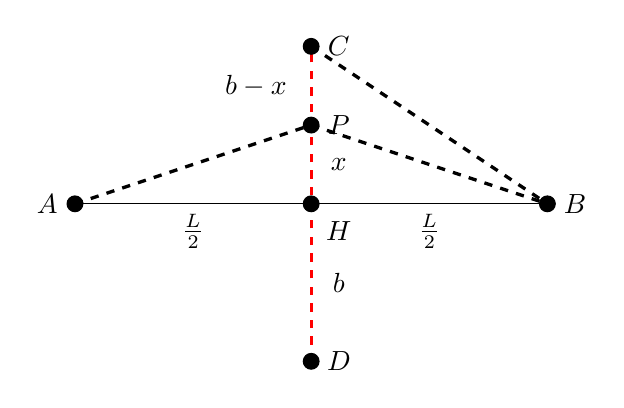
\begin{tikzpicture}
	\draw (0,0) to (6,0);
	\draw[red, very thick, dashed] (3,-2) to (3,2);
	\draw[very thick, dashed] (0,0) to (3,1);
	\draw[very thick, dashed] (3,1) to (6,0);
	\draw[very thick, dashed] (3,2) to (6,0);
	\draw[fill] (0,0) circle [radius=.1];
	\draw[fill] (6,0) circle [radius=.1];
	\draw[fill] (3,0) circle [radius=.1];
	\draw[fill] (3,2) circle [radius=.1];
	\draw[fill] (3,1) circle [radius=.1];
	\draw[fill] (3,-2) circle [radius=.1];
	\node[xshift=-10pt] at (0,0) {$A$} ;
	\node[yshift=-10pt] at (1.5,0) {$\frac{L}{2}$} ;
	\node[yshift=-10pt] at (4.5,0) {$\frac{L}{2}$} ;
	\node[xshift= 10pt] at (6,0) {$B$} ;
	\node[xshift= 10pt] at (3,2) {$C$} ;
	\node[xshift= -20pt] at (3,1.5) {$b-x$} ;
	\node[xshift= 10pt] at (3,1) {$P$} ;
	\node[xshift= 10pt] at (3,0.5) {$x$} ;
	\node[xshift= 10pt] at (3,-1) {$b$} ;
	\node[xshift= 10pt] at (3,-2) {$D$} ;
	\node[xshift= 10pt, yshift= -10pt] at (3,0) {$H$} ;
\end{tikzpicture}
\end{center}

By the assumption of the question, we know line segment $AB=L$ and the fence length is $2b$. We set point $C$ as upper endpoint of fence and $D$ as lower endpoint, then line segment $CD=2b$. Set point $H$ at where line segment $AB$ and fence $CD$ intersect. Then by assumption `electric fence in the exact middle of his daily path` and `it extends for a distance $b$ on each side of the path`, we know $AH=BH=\frac{L}{2}$ and $CH=DH=b$. We set point $P$ on the $CH$ to calculate length of the trip since point $P$ can be reflected by $AB$. Suppose $PH=x$ and we can get $CP=CH-PH=b-x$.

By Pythagoras Theorem, we know:
\begin{align*}
    PB=AP&=\sqrt{AH^2+PH^2} \quad(\mbox{Pythagoras Theorem})\\
    &=\sqrt{(\frac{L}{2})^2+x^2} \qquad \mbox{ for some } x\in[0,b] \quad(AH=\frac{L}{2} \mbox{ and } PH=x)
\end{align*}

By Pythagoras Theorem, we also know:
\begin{align*}
    BC&=\sqrt{CH^2+HB^2} \quad(\mbox{Pythagoras Theorem})\\
    &=\sqrt{b^2+(\frac{L}{2})^2}\quad(BH=\frac{L}{2} \mbox{ and } PH=b)
\end{align*}

If the electric fence is on, the length of the trip is:
\begin{align*}
    AP+PC+BC
    &=\sqrt{(\frac{L}{2})^2+x^2}+(b-x)+\sqrt{b^2+(\frac{L}{2})^2} \quad \mbox{ for some } x\in[0,b] \quad \circled{1}\\ &\quad(AP=\sqrt{(\frac{L}{2})^2+x^2}\mbox{ and }PC=b-x\mbox{ and }BC=\sqrt{b^2+(\frac{L}{2})^2})
\end{align*}

If the electric fence is off, the length of the trip is:
\begin{align*}
    AP+PB&=2AP \quad(AP=PB)\\
    &=2\sqrt{(\frac{L}{2})^2+x^2} \qquad \mbox{ for some } x\in[0,b] \quad(AP=\sqrt{(\frac{L}{2})^2+x^2}) \quad \circled{2}
\end{align*}

Then the average length represented by $f$ of the trip is:
\begin{align*}
    f(x)&=\frac{AP+PC+BC+AP+PB}{2}\\
    &=\frac{\sqrt{(\frac{L}{2})^2+x^2}+(b-x)+\sqrt{b^2+(\frac{L}{2})^2}+2\sqrt{(\frac{L}{2})^2+x^2}}{2} \quad\mbox{Total length is }\mbox{\circled{1} and \circled{2}}\\
    &=\frac{3\sqrt{(\frac{L}{2})^2+x^2}}{2}+\frac{b-x}{2}+\frac{\sqrt{b^2+(\frac{L}{2})^2}}{2} \quad\circled{3}
\end{align*}

Since the terms under square root are equal to or bigger than $0$, so $f$ are strictly positive and continuous on $[0,b]$. By Extreme Value Theorem, we know $f$ has a minimum on $[0,b]$, which we know must be a critical point or at an endpoint of the domain. $f$ is differentiable on $(0,b)\subseteq[0,b]$ and by implicit differentiation and \circled{3}, we want to find critical point:
\begin{align*}
    f'(x)
    &=\frac{3}{2}\cdot\frac{2x}{2\sqrt{(\frac{L}{2})^2+x^2}}-\frac{1}{2} \quad(\mbox{Chain Rule and Implicit Differentiation})\\
    &=\frac{3x}{2\sqrt{(\frac{L}{2})^2+x^2}}-\frac{1}{2}\\
\end{align*}
We want to find critical point, so we should let $f'(x) = 0$, which implies:
\begin{align*}
    \frac{3x}{2\sqrt{(\frac{L}{2})^2+x^2}}&=\frac{1}{2}\\
    3x&=\sqrt{(\frac{L}{2})^2+x^2}\\
    9x^2&=(\frac{L}{2})^2+x^2\\
    8x^2&=(\frac{L}{2})^2\\
    x&=\frac{\sqrt{2}}{8}L
\end{align*}

Since $x > 0$, the only critical point is $x=\frac{\sqrt{2}}{8}L$.

The table shows that $f$ is decreasing on the left side of critical point and $f$ is increasing on the right side of critical point. So $x=\frac{\sqrt{2}}{8}L$ is a local minimum.

\begin{tabular}{l|l|l|l}
\hline
$x$     & $0$            & $\frac{\sqrt{2}}{8}L$ & $L$                               \\
\hline
$f'(x)$ & $-\frac{1}{2}$ & $0$                   & $\frac{3\sqrt{5}}{5}-\frac{1}{2}$
\end{tabular}

However we know $x\in[0,b]$, we don't know the relationship between $L$ and $b$.

The answer should be splitted in to cases:
\begin{itemize}
    \item If $x=\frac{\sqrt{2}}{8}L\in [0,b]$, then point $P$ is $\frac{\sqrt{2}}{8}L$ up or down of point $H$.
    \item If $x=\frac{\sqrt{2}}{8}L>b$, since $f$ is decreasing when $x=\frac{\sqrt{2}}{8}L$, the minimum then is at $x=b$ as point $P$ is at $C$ or $D$.
    \item $x=\frac{\sqrt{2}}{8}L$ will never less than $0$ since $L>0$.
\end{itemize}

\newpage

\item  
	\begin{enumerate}
				
		\item  Let $f$ be a function with domain $\R$.  Assume $f$ has derivatives of every order.  Find all possible real numbers $A, B, C \in \R$ such that
			\begin{equation} \label{eq:ABC}
				\lim_{x \to 0} \frac{f(x) - \left[ Ax^2 + B x + C \right]}{x^2} = 0.
			\end{equation}	
			
			\emph{Note:} In your answer, $A$, $B$ and $C$ will depend on values of $f$ and its derivatives.  We are asking for \emph{all} possible answers.  We want you to prove that your choices of $A$, $B$, and $C$ satisfy \eqref{eq:ABC}, and that there are no other choices that satisfy \eqref{eq:ABC}.

			\emph{proof:}
			
			We want $\lim_{x \to 0} \frac{f(x) - (Ax^2 + Bx + C)}{x^2} = 0 \circled{1}$. 

			Since $\lim_{x \to 0} x^2 =0$, the only form possible is indeterminate form ($\lim_{x \to 0} f(x) - (Ax^2 + Bx + C) = 0$).
			Otherwise, this limit does not exist.

			Since $f$ has derivatives of every order, we can proof it is valid to use L'Hôpital's Rule. 
			Using L'Hôpital's Rule, we get:

			$$
				\lim_{x \to 0} \frac{f'(x) - (2Ax + B)}{2x} = 0 \circled{2}
			$$

			Same as above, $\lim_{x \to 0} 2x =0$, the only form possible is indeterminate form ($\lim_{x \to 0} f'(x) - (2Ax + B) = 0$).
			Otherwise, this limit does not exist. we can use L'Hôpital's Rule and get:

			$$
				\lim_{x \to 0} \frac{f''(x) - 2A}{2} = 0 \circled{3}
			$$

			Since $f$ has derivatives of every order, f is continuous on every order. 
			Thus, $\lim_{x \to 0} f''(x) = f''(0)$

			We can and only can take $A = \frac{f''(0)}{2}$ to satisfy the equation $\circled{3}$.

			Take the A back to $\circled{2}$, we get:

			$$
				\lim_{x \to 0} \frac{f'(x) - (2Ax + B)}{2x} = 0
			$$

			We have proven that $\lim_{x \to 0} f'(x) - (2Ax + B) = 0$. 
			Using limit laws, we can get $\lim_{x \to 0} f'(x) - \lim_{x \to 0} 2Ax - \lim_{x \to 0}B = 0$.

			Same as above, $\lim_{x \to 0} f'(x) = f'(0)$. Since $\lim_{x \to 0} 2Ax = 0$, 
			we can and only can take $B = f'(0)$.

			We have proven that $\lim_{x \to 0} f(x) - (Ax^2 + Bx + C) = 0$.
			Using limit laws, we can get $\lim_{x \to 0} f(x) - \lim_{x \to 0}Ax^2 - \lim_{x \to 0}Bx - \lim_{x \to 0}C = 0$.

			Same as above, $\lim_{x \to 0} f(x) = f(0)$. Since $\lim_{x \to 0}Ax^2 = 0$ and $\lim_{x \to 0}Bx = 0$, 
			we can and only can take $C = f(0)$.

			We have shown that $A = \frac{f''(0)}{2}, B = f'(0), C = f(0)$ can satisfy (1), and that there are no other choice that satisfy (1).
			% \begin{align*}
			% 	&\lim_{x \to 0} \frac{f(x) - (Ax^2 + Bx + C)}{x^2} \\
			% 	=&\lim_{x \to 0} \frac{f(x) - C - (Ax^2 + Bx)}{x^2} \\
			% 	=&\lim_{x \to 0} \frac{f(x) - C}{x^2} - \lim_{x \to 0} \frac{Ax^2}{x^2} + \lim_{x \to 0} \frac{Bx}{x^2} \\
			% \end{align*}

			% Thus we can conclude that
			% %%%%%%%%%%%%%%%%%%%%%%%%%%%
			% %%need more details here?%%
			% %%%%%%%%%%%%%%%%%%%%%%%%%%%
			% $$
			% 	\lim_{x \to 0} \frac{Ax^2}{x^2} =  A\lim_{x \to 0} \frac{x^2}{x^2} = 0
			% $$
			% % $$
			% % 	\lim_{x \to 0} \frac{Bx}{x^2} = B\lim_{x \to 0} \frac{x}{x^2} = 0
			% % $$

			% \begin{align*}
			% 	\lim_{x \to 0} f'(x) -2Ax-B &= 0\\
			% 	\lim_{x \to 0} \frac{f'(x)}{2x} - \lim_{x \to 0} \frac{f''(0)x}{2x} - \lim_{x \to 0} \frac{B}{2x} &= 0
			% \end{align*}


			% $\lim_{x \to 0} \frac{Ax^2}{x^2}$ %and $\lim_{x \to 0} \frac{Bx}{x^2}$ 
			% always equal to 0 for all $A, B \in \R$.

			% Since we want the original equation equals to 0, the equation can be rewritten as:

			% \begin{align*}
			% 	0=&\lim_{x \to 0} \frac{f(x) - C}{x^2} - \lim_{x \to 0} \frac{Ax^2}{x^2} + \lim_{x \to 0} \frac{Bx}{x^2}\\
			% 	0=&\lim_{x \to 0} \frac{f(x) - C}{x^2} - \lim_{x \to 0} \frac{Bx}{x^2} + 0\\
			% 	%0=&\lim_{x \to 0} \frac{f(x)}{x^2} - \lim_{x \to 0} \frac{C}{x^2} \\
			% \end{align*}
			
			% Because $f$ has derivatives of every order, $\lim_{x \to 0} f(x) = f(0)$. 
			% Thus we can get $C=f(0)$.

\newpage			

		\item  Let $f$ be a function with domain $\R$.  Assume $f$ has derivatives of every order.   Let $N$ be a positive integer.  Find a polynomial \DS{P_N} such that
			$$
				\lim_{x \to 0} \frac{f(x) - P_N(x)}{x^N} = 0
			$$
			\emph{Suggestion:} You may want to do some rough work until you can form a conjecture.    Do not submit the rough work.  To prove your conjecture, use induction.

			\emph{proof:}

			$$
			P_N = (\sum_{k = 1}^{N}\frac{f^k(0)}{k!}x^k) + f(0)
			$$

			I'll proof it using induction.

			\textbf{base step}: Assume N = 1.
			WTS:
			$$
				\lim_{x \to 0} \frac{f(x) - P_1(x)}{x} = 0
			$$

			We can write left hand of the equation as:

			\begin{align*}
				&\lim_{x \to 0} \frac{f(x) - f'(0)x - f(0)}{x} \\
				=& \lim_{x \to 0} \frac{f(x) - f(0) - f'(0)x}{x}
			\end{align*}

			Since $\lim_{x \to 0}{f(x) - f(0)} = 0, \lim_{x \to 0}{f'(0)x} = 0$, and  $f$ has derivatives of every order,
			we could use L'H\^{o}pital's Rule:

			$$
				\lim_{x \to 0} \frac{f(x) - f(0) - f'(0)x}{x}
				= \lim_{x \to 0} f'(x) - f'(0)
			$$

			Since $f$ has derivatives of every order, f is continuous on every order. 
			Thus, $\lim_{x \to 0} f'(x) = f'(0)$. 
			Take this back to the equation, we can get
			$$
				\lim_{x \to 0} f'(x) - f'(0) = 0
			$$
			which means 
			$$
				\lim_{x \to 0} \frac{f(x) - P_1(x)}{x} = 0
			$$

			\textbf{Induction step:}
			
			Assume $P_N$ satisfy $$\lim_{x \to 0} \frac{f(x) - P_N(x)}{x^N} = 0$$

			\emph{WTS:} $$\lim_{x \to 0} \frac{f(x) - P_{N+1}(x)}{x^{N+1}} = 0$$ 
			
			We can expand $P_{N+1}$, so the left hand side of the equation can be written as:

			\begin{align*}
				&\lim_{x \to 0} \frac{f(x) - \sum_{k = 1}^{N + 1} \frac{f^k(0)x^k}{k!} - f(0)}{x^{N + 1}} \\
				=& \lim_{x \to 0} \frac{f(x) - \sum_{k = 1}^{N} \frac{f^k(0)x^k}{k!} - f(0) - \frac{f^{N + 1}(0)x^{N + 1}}{(N + 1)!}}{x^{N + 1}} \\
			\end{align*}

			We know that
			\begin{itemize}
				\item $\lim_{x \to 0} f(x) = 0$
				\item $\lim_{x \to 0} \sum_{k = 1}^{N} \frac{f^k(0)x^k}{k!} = 0$
				\item $\lim_{x \to 0} f(0) = 0$
				\item $\lim_{x \to 0} \frac{f^{N + 1}(0)x^{N + 1}}{(N + 1)!} = 0$
			\end{itemize}

			And we can use L'H\^{o}pital's Rule $N + 1$ times.
			The highest power of $\sum_{k = 1}^{N} \frac{f^k(0)x^k}{k!}$ is $N$, and $N < N + 1$.
			So after $N + 1$ times of calculating derivatives, $\sum_{k = 1}^{N} \frac{f^k(0)x^k}{k!}$ becomes 0.
			$f(0)$ becomes 0 in the first calculating.

			$\lim_{x \to 0} \frac{f^{N + 1}(0)x^{N + 1}}{(N + 1)!} = 0$ after $N + 1$ times of calculating derivatives, 
			is $f^{N + 1}(0)$.

			the equation, after $N + 1$ times of calculating derivatives, is:

			$$
				\lim_{x \to 0} \frac{f^{N + 1}(x) - f^{N + 1}(0)}{(N + 1)!}
			$$

			Since $f$ has derivatives of every order, f is continuous on every order. 
			Thus, $\lim_{x \to 0} f^{N + 1}(x) = f^{N + 1}(0)$. 

			This means $\lim_{x \to 0} f^{N + 1}(x) - f^{N + 1}(0) = 0$, which indicates that 
			$$\lim_{x \to 0} \frac{f(x) - P_{N+1}(x)}{x^{N+1}} = 0$$
			

		\item  Using your new result, find polynomials $P$  and $Q$ such that
			$$
				\lim_{x \to 0} \frac{e^x - P(x)}{x^6} = 0, \quad \quad \lim_{x \to 0} \frac{\sin x - Q(x)}{x^{11}} = 0.
			$$
	\end{enumerate}

\vv

\emph{Proof:}

\vv

We know that derivative of $e^x$ is $e^x$ which is as same as itself. Then we get the information that $f(x)=e^x$ has derivatives of every order.

For the first equation $$\lim_{x\to0}\frac{e^x-P(x)}{x^6}=0$$
We take $N=6$ and we can then apply the formula into $$\lim_{x \to 0} \frac{f(x) - P_N(x)}{x^N} = 0$$ By using
$$P_N = (\sum_{k = 1}^{N}\frac{f^k(0)}{k!}x^k) + f(0).$$ And we get and expand this polynomial:
\begin{align*}
    P(x)=P_6 &= (\sum_{k = 1}^{6}\frac{f^k(0)}{k!}x^k) + f(0).\\
    &=\frac{f^6(0)}{6!}x^6+\frac{f^5(0)}{5!}x^5+\frac{f^4(0)}{4!}x^4+\frac{f^3(0)}{3!}x^3+\frac{f^2(0)}{2!}x^2+\frac{f'(0)}{1!}x+f(0)\quad()\\
    &=\frac{1}{6!}x^6+\frac{1}{5!}x^5+\frac{1}{4!}x^4+\frac{1}{3!}x^3+\frac{1}{2!}x^2+\frac{1}{1!}x+1\quad(\frac{d}{dx}e^x=e^x\mbox{ and }e^0=1)\\
    &=\frac{x^6}{6!}+\frac{x^5}{5!}+\frac{x^4}{4!}+\frac{x^3}{3!}+\frac{x^2}{2!}+x+1
\end{align*}

We know that:
\begin{align*}
    &\frac{d}{dx}\sin{x}=\cos{x}\\
    &\frac{d}{dx}\cos{x}=-\sin{x}\\
    &\frac{d}{dx}-\sin{x}=-\cos{x}\\
    &\frac{d}{dx}-\cos{x}=\sin{x}
\end{align*}
Then we get the information that $f(x)=\sin{x}$ has derivatives of every order and $f^N(x)=f^{N+4}(x)$.

For the second equation $$\lim_{x \to 0} \frac{\sin x - Q(x)}{x^{11}} = 0$$
We take $N=11$ and we can then apply the formula into $$\lim_{x \to 0} \frac{f(x) - P_N(x)}{x^N} = 0$$ By using
$$P_N = (\sum_{k = 1}^{N}\frac{f^k(0)}{k!}x^k) + f(0).$$ And we get and expand this polynomial:
\begin{align*}
    Q(x)=P_{11} =& (\sum_{k = 1}^{11}\frac{f^k(0)}{k!}x^k) + f(0).\\
    =&\frac{f^{11}(0)}{11!}x^{11}+\frac{f^{10}(0)}{10!}x^{10}+\frac{f^9(0)}{9!}x^9+\frac{f^8(0)}{8!}x^8+\frac{f^7(0)}{7!}x^7+\frac{f^6(0)}{6!}x^6+\frac{f^5(0)}{5!}x^5+\\
    &\frac{f^4(0)}{4!}x^4+\frac{f^3(0)}{3!}x^3+\frac{f^2(0)}{2!}x^2+\frac{f^1(0)}{1!}x+f(0)\quad(\mbox{Expand Sum Formula})\\
    =&\frac{-\cos{0}}{11!}x^{11}+\frac{-\sin{0}}{10!}x^{10}+\frac{\cos{0}}{9!}x^9+\frac{\sin{0}}{8!}x^8+\frac{-\cos{0}}{7!}x^7+\frac{-\sin{0}}{6!}x^6+\frac{\cos{0}}{5!}x^5+\\
    &\frac{\sin{0}}{4!}x^4+\frac{-\cos{0}}{3!}x^3+\frac{-\sin{0}}{2!}x^2+\frac{\cos{0}}{1!}x+f(0)\quad(f^N(x)=f^{N+4}(x))\\
    =&\frac{-1}{11!}x^{11}+\frac{1}{9!}x^9+\frac{-1}{7!}x^7+\frac{1}{5!}x^5+\frac{-1}{3!}x^3+\frac{1}{1!}x\quad(\cos{0}=1\mbox{ and }\sin{0}=0)\\
    =&-\frac{x^{11}}{11!}+\frac{x^9}{9!}-\frac{x^7}{7!}+\frac{x^5}{5!}-\frac{x^3}{3!}+x
\end{align*}

We have found polynomials $P$ and $Q$ by our result from Q2b as needed. $\qquad\blacksquare$

\newpage

\vv

\item  In Video 6.13, you learned about various geometrical notions that we could have used to define concavity.  Here is yet another one.

 Let $f$ be a function defined on an interval $I$.  Given two points $P$ and $Q$ on the graph of $f$, we will call $m_{P,Q}$ the slope of the line going through $P$ and $Q$.  We say that the function $f$ is ``cave up" on $I$ when for every 3 different points $P$, $Q$, and $R$ on the graph of $f$, if $P$ is to the left of $Q$, and $Q$ is to the left of $R$, then $m_{P,Q} < m_{Q,R}$.  Sketch a graph and make sure you understand this definition geometrically  before continuing.
 
 Assume $f$ is differentiable on $I$. 
		Prove that IF $f$ is concave up on $I$, THEN $f$ is cave up on $I$.


\emph{Hint:}  Use MVT.

\emph{Note:}  It is also possible to prove that cave up implies concave up, but we will skip it for now.  In fact, all of the different versions of concavity you have learned are equivalent for differentiable functions.	

\vv

\emph{Proof:}

\vv

WTS: $f$ is concave up on $I \implies f$ is cave up on $I$

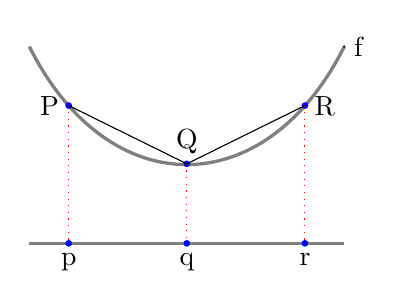
\begin{tikzpicture}

	\draw[gray, very thick] (-2, 2) .. controls (-1,0) and (1,0) .. (2, 2);
	\filldraw[black] (2, 2) circle (0.1pt) node[anchor=west] {f};
	\filldraw[blue] (-1.5, 1.25) circle (1pt) node[anchor=east, black] {P};
	\filldraw[blue] (0, 0.51) circle (1pt) node[anchor=south, black] {Q};
	\filldraw[blue] (1.5, 1.25) circle (1pt) node[anchor=west, black] {R};
	\draw (-1.5, 1.25) -- (0, 0.51);
	\draw (0, 0.51) -- (1.5, 1.25);

	\draw[gray, very thick] (-2, -0.5) -- (2, -0.5);
	\draw[red, dotted] (-1.5, 1.25) -- (-1.5, -0.5);
	\draw[red, dotted] (0, 0.51) -- (0, -0.5);
	\draw[red, dotted] (1.5, 1.25) -- (1.5, -0.5);

	\filldraw[blue] (-1.5, -0.5) circle (1pt) node[anchor=north, black] {p};
	\filldraw[blue] (0, -0.5) circle (1pt) node[anchor=north, black] {q};
	\filldraw[blue] (1.5, -0.5) circle (1pt) node[anchor=north, black] {r};

\end{tikzpicture}


We assume function $f$ is concave up on an interval $I$.

Let $P, Q, R$ on the graph of $f$. Assume $P$ is to the left of $Q$, and $Q$ is to the left of $R$. Assume $p, q, r \in I$ represent the x-coordinates of $P, Q, R$.
We need to show that $m_{P,Q}=\frac{f(q)-f(p)}{q-p}<m_{Q,R}=\frac{f(r)-f(q)}{r-q}$.

By the definition of "$f$ is concave up on $I$ ", we know that $f$ is differentiable on $I$ and then implies $f$ is continuous on $I$.

We know that $(p,q)\subseteq I \land [p,q]\subseteq I$, then we can get $f$ is continuous on $[p,q]$ and differentiable on $(p,q)$.

By Mean Value Theorem, we know that $\exists m_1\in(p,q)$ s.t.
$$
    f'(m_1)=\frac{f(q)-f(p)}{q-p}
$$

We also know that $(q,r)\subseteq I \land [q,r]\subseteq I$, then we can get $f$ is continuous on $[q,r]$ and differentiable on $(q,r)$.

By Mean Value Theorem, we know that $\exists m_2\in(q,r)$ s.t.
$$
    f'(m_2)=\frac{f(r)-f(q)}{r-q}
$$

It's very easy to know that $m_1\in(p,q)$ and $m_2\in(q,r)$ can imply $p<m_1<q$ and $q<m_2<r$. Then we can get the conclusion that $m_1<q<m_2$.

By the definition of "$f$ is concave up on $I$ ", we know that $f'$ is increasing on $I$. By the definition of increasing: '$\forall x_1, x_2\in I, x_1<x_2 \implies f(x_1)<f(x_2)$', let $x_1=m_1 \land x_2=m_2 \land x_1=m_1<m_2=x_2$, we can imply that $f'(m_1)<f'(m_2)$.

We have proven that $m_{P,Q}=f'(m_1)=\frac{f(q)-f(p)}{q-p} < \frac{f(r)-f(q)}{r-q}=f'(m_2)=m_{Q,R}. \qquad\blacksquare$

\newpage

\item  Let's recall the definition of horizontal/slant asymptote.  Let $f$ be a function defined at least on an interval $(c,\infty)$ for some $c \in \R$.
We say that $f$ has an asymptote as $x \to \infty$ when there exist numbers $m, b \in \R$ such that
	$$	
		\lim_{x \to \infty} \left[ f(x) - \left( mx + b \right) \right] \; = \; 0.
	$$
Notice that this includes both slant asymptotes (when $m \neq 0$) and horizontal asymptotes (when $m =0$).
	
Consider the following two claims:	
			\begin{center}
				{\bf Claim A:} \quad \quad
					IF $f$ has an asymptote as $x \to \infty$,  \quad
					THEN \DS{\lim_{x \to \infty} \frac{f(x)}{x}} exists.
				
				{\bf Claim B:} \quad \quad 		
					IF \DS{\lim_{x \to \infty} \frac{f(x)}{x}} exists, \quad
					THEN $f$ has an asymptote as $x \to \infty$.
			\end{center}
	\begin{enumerate}
		\item Prove that Claim A is true.
		
		\vv
		
		\emph{Proof:}
		
		\vv
		
		We assume that $f$ has an asymptote as $x \to \infty$. This means $\exists m,b\in\R$ such that:
		$$
		    \lim_{x \to \infty} \left[ f(x) - \left( mx + b \right) \right] \; = \; 0 \quad\circled{4}
		$$
		We can find out that:
		\begin{align*}
		    \lim_{x \to \infty} \frac{f(x)}{x}
		    &=\lim_{x \to \infty} (\frac{f(x)-mx+mx-b+b}{x})\\
		    &=\lim_{x \to \infty} (\frac{f(x)-mx-b}{x}+m+\frac{b}{x}) \quad (x \to \infty \implies x \neq 0)\\
		    &=\lim_{x \to \infty}(\frac{f(x)-mx-b}{x})+m+\lim_{x \to \infty}(\frac{b}{x}) \quad(\mbox{By Limit Law of Sum})\\
		    &=\lim_{x \to \infty}(\frac{f(x)-mx-b}{x})+m+0\quad(\lim_{x \to \infty}(\frac{b}{x})=0)\\
		    &=\lim_{x \to \infty}[\frac{f(x)-(mx+b)}{x}]+m \quad \circled{*}
		\end{align*}
		As we know that $\lim_{x \to \infty}x=\infty$ and $\circled{*}$ is True, we can then continue to calculate the limit. 
		
		Using limit law of quotient, we can write $\circled{*}$ as:
		$$
		    \lim_{x \to \infty} \frac{f(x)}{x}=\frac{\lim_{x \to \infty}[f(x)-(mx+b)]}{\lim_{x \to \infty}x}+m=0+m=m
		$$
		So, $\lim_{x \to \infty} \frac{f(x)}{x}$ exists and equals to $m$. Thus we have proven that Claim A.$\quad\blacksquare$
		
		\newpage
		
		\item Prove that Claim B is false.
		
		\vv
		
		\emph{Proof:}
		
		\vv
		
		Since we need to prove the Claim B is false, I will give a counterexample. Let $f(x)=x+\cos{x}.$
		Then we can get equation:
		\begin{align*}
		    \lim_{x \to \infty} \frac{f(x)}{x}&=\lim_{x \to \infty}(\frac{x+\cos{x}}{x}) \\
		    &=\lim_{x \to \infty}(\frac{x}{x}+\frac{\cos{x}}{x})\quad (x \to \infty \implies x \neq 0)
		\end{align*}
		
		Since
		\begin{align*}
		    -1\leq&\cos{x}\leq1\\
		    -\frac{1}{x}\leq&\frac{\cos{x}}{x}\leq\frac{1}{x}
		\end{align*}
		
		We can calculate that $\lim_{x \to \infty}-\frac{1}{x}=\lim_{x \to \infty}\frac{1}{x}=0$. By Squeeze Theorem, we know that $\lim_{x \to \infty}(\frac{\cos{x}}{x})=0$. Thus by Limit Law of Sum,
		$$
		    \lim_{x \to \infty} \frac{f(x)}{x}=\lim_{x \to \infty}(\frac{x}{x})+\lim_{x \to \infty}(\frac{\cos{x}}{x})=1+0=1
		$$
		We now get the assumption $\lim_{x \to \infty}$ exists. Then we need to prove $f$ doesn't have an asymptote as $x \to \infty$.
		
		WTS:$\forall m,b\in\R,\lim_{x \to \infty}[f(x)-(mx+b)]\neq0.$
		
		Let $m,b\in\R.$
		
		Cases:
		\begin{itemize}
		    \item When $m=1$, we can get:
		    \begin{align*}
		        \lim_{x \to \infty}[f(x)-(mx+b)]&=\lim_{x \to \infty}[x+\cos{x}-x-b]\quad(f(x)=x+\cos{x})\\
		        &=\lim_{x \to \infty}[\cos{x}-b]
		    \end{align*}
		    Since $\lim_{x \to \infty}\cos{x}$ did not exists and $\lim_{x \to \infty}b$ is a constant, by limit law of sum, the answer of whole equation is D.N.E.
		    \item When $m\neq1$, we can get:
		    \begin{align*}
		        \lim_{x \to \infty}[f(x)-(mx+b)]&=\lim_{x \to \infty}[x+\cos{x}-mx-b]\quad(f(x)=x+\cos{x})\\
		        &=\lim_{x \to \infty}[(1-m)x+\cos{x}-b]\\
		        &=\lim_{x \to \infty}[x\cdot(1-m+\frac{\cos{x}}{x}-\frac{b}{x})] \quad\circled{5}
		    \end{align*}
		    By the Limit Law of Sum,
		    \begin{align*}
				&\lim_{x \to \infty}(1-m+\frac{\cos{x}}{x}-\frac{b}{x})\\
				&=\lim_{x \to \infty}(1-m)+\lim_{x \to \infty}(\frac{\cos{x}}{x})-\lim_{x \to \infty}(\frac{b}{x}) \quad (x \to \infty \implies x \neq 0)\\
		        &=1-m+0+0\quad(\lim_{x \to \infty}(\frac{\cos{x}}{x})=0\mbox{ and }\lim_{x \to \infty}(\frac{b}{x})=0)\\
		        &=1-m
		    \end{align*}
		    We know that when $m\neq1$, it can imply $1-m\neq1+(-1)=0$. 
		    
		    Back to \circled{5}, we now know $\lim_{x \to \infty}x=\infty$ and $\lim_{x \to \infty}(1-m+\frac{\cos{x}}{x}-\frac{b}{x})$ is non-zero, then...
		    
		    When $m<1$, $\lim_{x \to \infty}(1-m+\frac{\cos{x}}{x}-\frac{b}{x})=1-m>0$, we can get:
		    \begin{align*}
		        \lim_{x \to \infty}[f(x)-(mx+b)]&=\lim_{x \to \infty}[x\cdot(1-m+\frac{\cos{x}}{x}-\frac{b}{x})]\\
		        &=\infty\quad(\mbox{Limit Law of Product})
		    \end{align*}
		    When $m>1$, $\lim_{x \to \infty}(1-m+\frac{\cos{x}}{x}-\frac{b}{x})=1-m<0$, we can get:
		    \begin{align*}
		         \lim_{x \to \infty}[f(x)-(mx+b)]&=\lim_{x \to \infty}[x\cdot(1-m+\frac{\cos{x}}{x}-\frac{b}{x})]\\
		        &=-\infty\quad(\mbox{Limit Law of Product})
		    \end{align*}
		\end{itemize}
		We have proven that $\lim_{x \to \infty}[f(x)-(mx+b)]\neq0$ as needed. $\qquad\blacksquare$
		
		\newpage
		
		\item  Here is one more false claim and a bad proof.
			\begin{quotation}
				\noindent
				{\bf Claim C:} Assume the function $f$ is differentiable and that \DS{\lim_{x \to \infty} f(x) = \infty}.
				
				$$  \lim_{x \to \infty} \frac{f(x)}{x} \mbox{ exists} \quad \iff \quad \lim_{x \to \infty} f'(x) \mbox{ exists } $$
				
				
				\noindent
				{\bf ``Proof":}  We can use L'H\^{o}pital's Rule:
					$$
						\lim_{x \to \infty} \frac{f(x)}{x} \; = \; \lim_{x \to \infty} \frac{\frac{d}{dx} f(x)}{\frac{d}{dx} x} 
							\; = \; \lim_{x \to \infty} \frac{f'(x)}{1} \; = \; \lim_{x \to \infty} f'(x)
					$$
					\ \hfill $\square$
			\end{quotation}
			Explain the  error in the proof.
			
			Then prove that the claim is false with a counterexample.
			
			\vv
			
			\emph{Problem:}
			
			\vv
			
			The error in this question is obvious; The author of this faulty proof uses L'H\^{o}pital's Rule without showing the preconditions for L'H\^{o}pital's Rule.
			
			Here is L'H\^{o}pital's Rule in Video 6.6:
			
			IF
			\begin{itemize}
			    \item i. $f$ and $g$ are differentiable as $x \to a$.
			    \item ii. $g$ and $g'$ are never $0$ as $x \to a$.
			    \item iii. The limit $\lim_{x \to a}\frac{f(x)}{g(x)}$ is an indeterminate form of type $\frac{0}{0}$ or $\frac{\pm\infty}{\pm\infty}$
			    \item iv. The limit $\lim_{x \to a}\frac{f'(x)}{g'(x)}$ exists or is $\infty$ or $-\infty$
			    
			\end{itemize}
			THEN
			$$
			    \lim_{x \to a}\frac{f(x)}{g(x)}=\lim_{x \to a}\frac{f'(x)}{g'(x)}.
			$$
			
			In his proof, we do not know what the value of $f$ and the existence of $f'$  when the limit tends to infinity. This leads to it may not satisfy the iii) and iv) of L'H\^{o}pital's Rule assumptions. Then we can't apply L'H\^{o}pital's Rule.
			
			\emph{Counterexample:}
			
			Let $f(x)=x+\sin{x}$.
			
			We know $f(x)$ is diffrentiable on $\R$.
			And $\lim_{x \to \infty}(x+\sin{x})=\infty$ can to be proven by Squeeze Theorem as
			\begin{align*}
			    -1\leq&\sin{x}\leq 1\\
			    x-1\leq&x+\sin{x}\leq x+1
			\end{align*}
			We know $\lim_{x \to \infty}(x-1)=\lim_{x \to \infty}(x+1)=\infty$, then we have proven $\lim_{x \to \infty}(x+\sin{x})=\infty$ \circled{6}
			
			When $\lim_{x \to \infty}\frac{f(x)}{g(x)}=\lim_{x \to \infty}\frac{x+\sin{x}}{x}$, we will find out that,
			$$
			    \lim_{x \to \infty}(x+\sin{x})'=\lim_{x \to \infty}(1+\cos{x})\quad(\sin'(x)=\cos{x})
			$$
			We know that $\lim_{x \to \infty}1$ is a constant and $\lim_{x \to \infty}\cos{x}$ doesn't exist \circled{7}. So we can't use L'H\^{o}pital's Rule.
			
			\emph{Proof:}

			WTS: $\exists f, \lim_{x \to \infty} \frac{f(x)}{x} \mbox{ exists} \quad \land \quad \lim_{x \to \infty} f'(x) \mbox{ does not exists }$
			
			Also take $f(x)=x+\sin{x}$ as counterexample.
			We know $f(x)$ is diffrentiable on $\R$ and $\lim_{x \to \infty}(x+\sin{x})=\infty$. \circled{6}
			\begin{align*}
			    \lim_{x \to \infty}\frac{f(x)}{x}&=\lim_{x \to \infty}\frac{x+\sin{x}}{x}\quad(f(x)=x+\sin{x})\\
			    &=\lim_{x \to \infty}(1+\frac{\sin{x}}{x})
			\end{align*}
			Since
		    \begin{align*}
		        -1\leq&\sin{x}\leq1\\
		        -\frac{1}{x}\leq&\frac{\sin{x}}{x}\leq\frac{1}{x}
		     \end{align*}
		
		    We can calculate that $\lim_{x \to \infty}-\frac{1}{x}=\lim_{x \to \infty}\frac{1}{x}=0$. By Squeeze Theorem, we know that $\lim_{x \to \infty}(\frac{\sin{x}}{x})=0$. Thus by     Limit Law of Sum,
		    $$
		        \lim_{x \to \infty} \frac{f(x)}{x}=\lim_{x \to \infty}(1)+\lim_{x \to \infty}(\frac{\sin{x}}{x})=1+0=1
		    $$
			We have proven that $\lim_{x \to \infty} \frac{f(x)}{x}$ exists.
			
			Let's inspect $f'$ next. By Implicit differentiation, $f'(x)=(x+\sin{x})'=1+\cos{x}$.
		    
			The limit of $f'$, $\lim_{x \to \infty}f'(x)=\lim_{x \to \infty}(1+\cos{x})$, as we proven previously at \circled{7}, doesn't exist.
			
			To conclude:
		    $$
				\exists f, \lim_{x \to \infty} \frac{f(x)}{x} \mbox{ exists} \quad \land \quad \lim_{x \to \infty} f'(x) \mbox{ does not exists }
		    $$
		    Thus, we have proven Claim C is false. $\qquad\blacksquare$
		    
	\end{enumerate}

\end{enumerate}


\end{document}

%%%%%%%%%%%%%%%%%%%%%%%%%%%%%%%%%%%%%%%
%%%%%%%%%%%%%%%%%%%%%%%%%%%%%%%%%%%%%%%
%%%%%%%%%%%%%%%%%%%%%%%%%%%%%%%%%%%%%%%


	
